\documentclass[11pt,a4paper]{article}
\usepackage[T1]{fontenc}
\usepackage[utf8]{inputenc}
\usepackage[english]{babel}
\usepackage{lmodern}
\usepackage[margin=2.2cm]{geometry}
\usepackage{graphicx}
\usepackage{booktabs}
\usepackage{caption}
\usepackage{float}
\usepackage{amsmath}
\usepackage{tikz}
\usetikzlibrary{arrows.meta,positioning}
\usepackage[hidelinks]{hyperref}
\captionsetup{font=small,labelfont=bf}
\setlength{\parskip}{3pt}

\newcommand{\nphotos}{173}
\newcommand{\nnests}{49}
\newcommand{\npairs}{25}
\newcommand{\nmanual}{72}
\newcommand{\nauto}{101}
\newcommand{\scaleboth}{14}
\newcommand{\scaledev}{0.2}
\newcommand{\scaledevmax}{0.8}
\newcommand{\areamed}{317}
\newcommand{\areamin}{126}
\newcommand{\areamax}{651}
\newcommand{\nmix}{104}
\newcommand{\nmixnests}{37}
\newcommand{\medmixthree}{0.30}
\newcommand{\medmixtwelve}{0.66}
\newcommand{\medmixfortyeight}{0.91}
\newcommand{\medcellsix}{0.29}
\newcommand{\medcellhundred}{0.88}
\newcommand{\nestmixmin}{0.21}
\newcommand{\nestmixmax}{0.87}
\newcommand{\nestmixn}{37}
\newcommand{\spearmixcell}{0.95}
\newcommand{\centorange}{0.28}
\newcommand{\centyellow}{0.40}
\newcommand{\centwhite}{0.28}
\newcommand{\centred}{0.39}
\newcommand{\centblack}{0.42}
\newcommand{\exAmix}{0.38}
\newcommand{\exAcell}{0.27}
\newcommand{\exAhet}{0.54}
\newcommand{\exBmix}{0.86}
\newcommand{\exBcell}{0.65}
\newcommand{\exBhet}{0.51}
\newcommand{\valn}{370}
\newcommand{\valnunsure}{34}
\newcommand{\valpunsure}{9}
\newcommand{\valnuniform}{189}
\newcommand{\valacc}{0.92}
\newcommand{\valacclo}{0.87}
\newcommand{\valacchi}{0.95}
\newcommand{\valaccstring}{0.93}
\newcommand{\valcolourok}{0.99}
\newcommand{\valncolour}{115}
\newcommand{\vallost}{2}
\newcommand{\valworst}{0.82}
\newcommand{\rhomean}{0.11}
\newcommand{\rholo}{0.07}
\newcommand{\rhohi}{0.15}
\newcommand{\rhopos}{61}
\newcommand{\rhon}{144}


\title{Colour mixing in zebra finch nests from top-view photographs\\[2pt]
\large Pipeline, validation and first results}
\author{Nest weave quantif project}
\date{26 November 2026}

\begin{document}
\maketitle

\begin{abstract}
Pairs of zebra finches built their nests with pieces of string given in a fixed colour sequence
(orange, yellow, white, then red, or black in one group, from the first egg on), so colour marks
the building phase. We measured, on \nphotos{} top-view photographs of \nnests{} nests built by
\npairs{} pairs, how the colours are arranged. Every pixel is classified by a two-stage random
forest trained on hand-drawn rectangles. On \valn{} blindly annotated random points from 16 pairs
that were never used for training, the classification is correct for \valacc{} of points
[95\,\% CI \valacclo--\valacchi] and gets the colour right for \valcolourok{} of string points.
Colours form patches of a few centimetres. Mixing varies a lot from nest to nest (median per nest from
\nestmixmin{} to \nestmixmax{}, where 0 means separate patches and 1 means random), but a pair does not
mix the same way in its two nests. Second nests tend to be slightly more mixed, at every scale, but the
effect is small and not robust. Later colours lie slightly
closer to the centre of the cup. The top view only shows the last layer of string, which limits
what it can say about stratification.
\end{abstract}

\section{Data}

\paragraph{Protocol.} Strings were given in bundles of 150 pieces: orange two days after pairing,
then yellow, then white, each when the previous colour ran out. As soon as the first egg was laid, the
birds switched directly to the last colour, whatever colour they had reached. After the first egg they
received no more string in cohort~1 round~1, black string in cohort~2 round~1, and red string in all
other cohort $\times$ round groups. Yellow and white can therefore be missing from a nest. Each pair built two nests
(rounds 1 and 2). The nests were photographed from the top, left and right at several sessions during
building, in a light box with a ruler card (Table~\ref{tab:groups}). This report uses the top views
only.

\begin{table}[H]
\centering\small
\begin{tabular}{ccccccc}
\toprule
cohort & round & pairs & nests & top views & colour after 1st egg & views with mixing defined \\
\midrule
\csname @@input\endcsname tables/groups.tex 
\bottomrule
\end{tabular}
\caption{Data set. Mixing is only computed when a second colour makes up at least 10\,\% of the
visible string (Section~\ref{sec:metrics}). In cohort~1 round~1 one colour usually covers the whole
top, so that group hardly enters the mixing analyses.}
\label{tab:groups}
\end{table}

\paragraph{Inventory.} The photo files were matched to nests and sessions automatically, from file
names and dates. Cohort~1 round~1 photos carry random three-digit codes and were matched with Marie's
correspondence table. Duplicate files and entrance views were excluded. A round is the set of sessions
of a pair that are less than 45 days apart.

\section{Processing pipeline}

\begin{figure}[H]
\centering
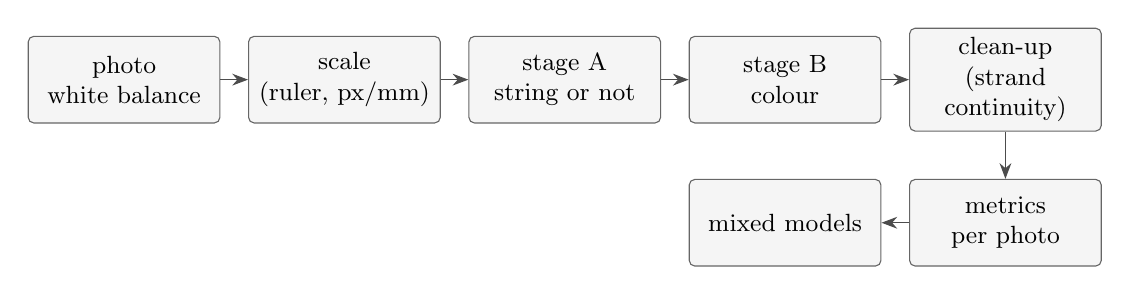
\begin{tikzpicture}[
  node distance=3.5mm,
  box/.style={draw=black!60, rounded corners=2pt, fill=black!4, align=center, font=\small,
              minimum height=11mm, text width=22mm},
  arr/.style={-{Stealth[length=2mm]}, black!70}]
\node[box] (p) {photo\\white balance};
\node[box, right=of p] (s) {scale\\(ruler, px/mm)};
\node[box, right=of s] (a) {stage A\\string or not};
\node[box, right=of a] (b) {stage B\\colour};
\node[box, right=of b] (c) {clean-up\\(strand continuity)};
\node[box, below=6mm of c] (m) {metrics\\per photo};
\node[box, left=of m] (st) {mixed models};
\draw[arr] (p) -- (s); \draw[arr] (s) -- (a); \draw[arr] (a) -- (b); \draw[arr] (b) -- (c);
\draw[arr] (c) -- (m); \draw[arr] (m) -- (st);
\end{tikzpicture}
\caption{Processing of one photograph.}
\label{fig:pipeline}
\end{figure}

\paragraph{Scale.} Each photo contains a ruler graduated every 10\,mm. The scale is detected
automatically by finding the regular rows of the ruler. A quality check rejects fits with too few
rows, an irregular spacing, or a value far from what the camera focal length predicts. Rejected or
hidden rulers were measured by hand in an annotation page (two clicks on visible graduations).
All \nphotos{} photos have a scale: \nauto{} automatic, \nmanual{} manual. Where both exist
(\scaleboth{} photos), they agree to \scaledev\,\% (median; maximum \scaledevmax\,\%). The ruler stands
slightly in front of the nest, so absolute sizes in mm are approximate to a few percent.

\paragraph{Segmentation.} A pixel classifier assigns every pixel to one of eight classes:
background, other material (wooden box, cardboard, ruler, eggs, feathers), gap / shadow, and the five
string colours. It works in two stages. Stage~A decides whether a pixel is string, from its
neighbourhood at several scales (texture, edges). Stage~B decides the colour of string pixels, from
local colour descriptors. Both stages are random forests: sets of decision trees, trained on examples,
that vote. A string pixel much darker than its colour's typical brightness is relabelled gap /
shadow. Finally, a clean-up step removes small colour islands that no strand explains, and bridges
short gaps along a strand.

\paragraph{Training data.} The examples are rectangles drawn by hand on 22 photos, each given a class:
581 by Marie on 19 photos, 39 by Renaud on 4 photos (mainly dense black string and dark gaps), and older
rectangles from the first data set. Inside a rectangle only pixels compatible with the class are kept,
for example sufficiently saturated pixels in a ``yellow'' rectangle. Every class is given the same
total weight, whatever its number of pixels. All training photos come from 9 pairs. The other 16 pairs
are kept apart for validation.

\paragraph{Model development.} Successive versions were compared on the 367 points of an earlier blind
validation (old data set, no black string; Table~\ref{tab:versions}). Adding Marie's rectangles and
balancing the classes improved accuracy. The new black class first confused dark gaps with black
string, which was fixed by adding gap / shadow rectangles. Version v7f is the one used here.
Figure~\ref{fig:examples} shows its output on photos of validation pairs.

\begin{table}[H]
\centering\small
\begin{tabular}{llccc}
\toprule
version & training data & accuracy & colour correct & black recognised \\
\midrule
v5b & old rectangles & 0.80 & 0.91 & no class \\
v6 & old rectangles, corrected hue limits & 0.84 & 0.95 & no class \\
v7c & + Marie's rectangles, balanced classes & 0.89 & 0.98 & only isolated strands \\
v7f & + dense black and gap rectangles & 0.86 & 0.98 & yes (0 false black points) \\
\bottomrule
\end{tabular}
\caption{Model versions, scored on the 367 points of the old data set. v7c scores higher on these points
but labels dense black nests as ``other material''; v7f handles both.}
\label{tab:versions}
\end{table}

\begin{figure}[p]
\centering
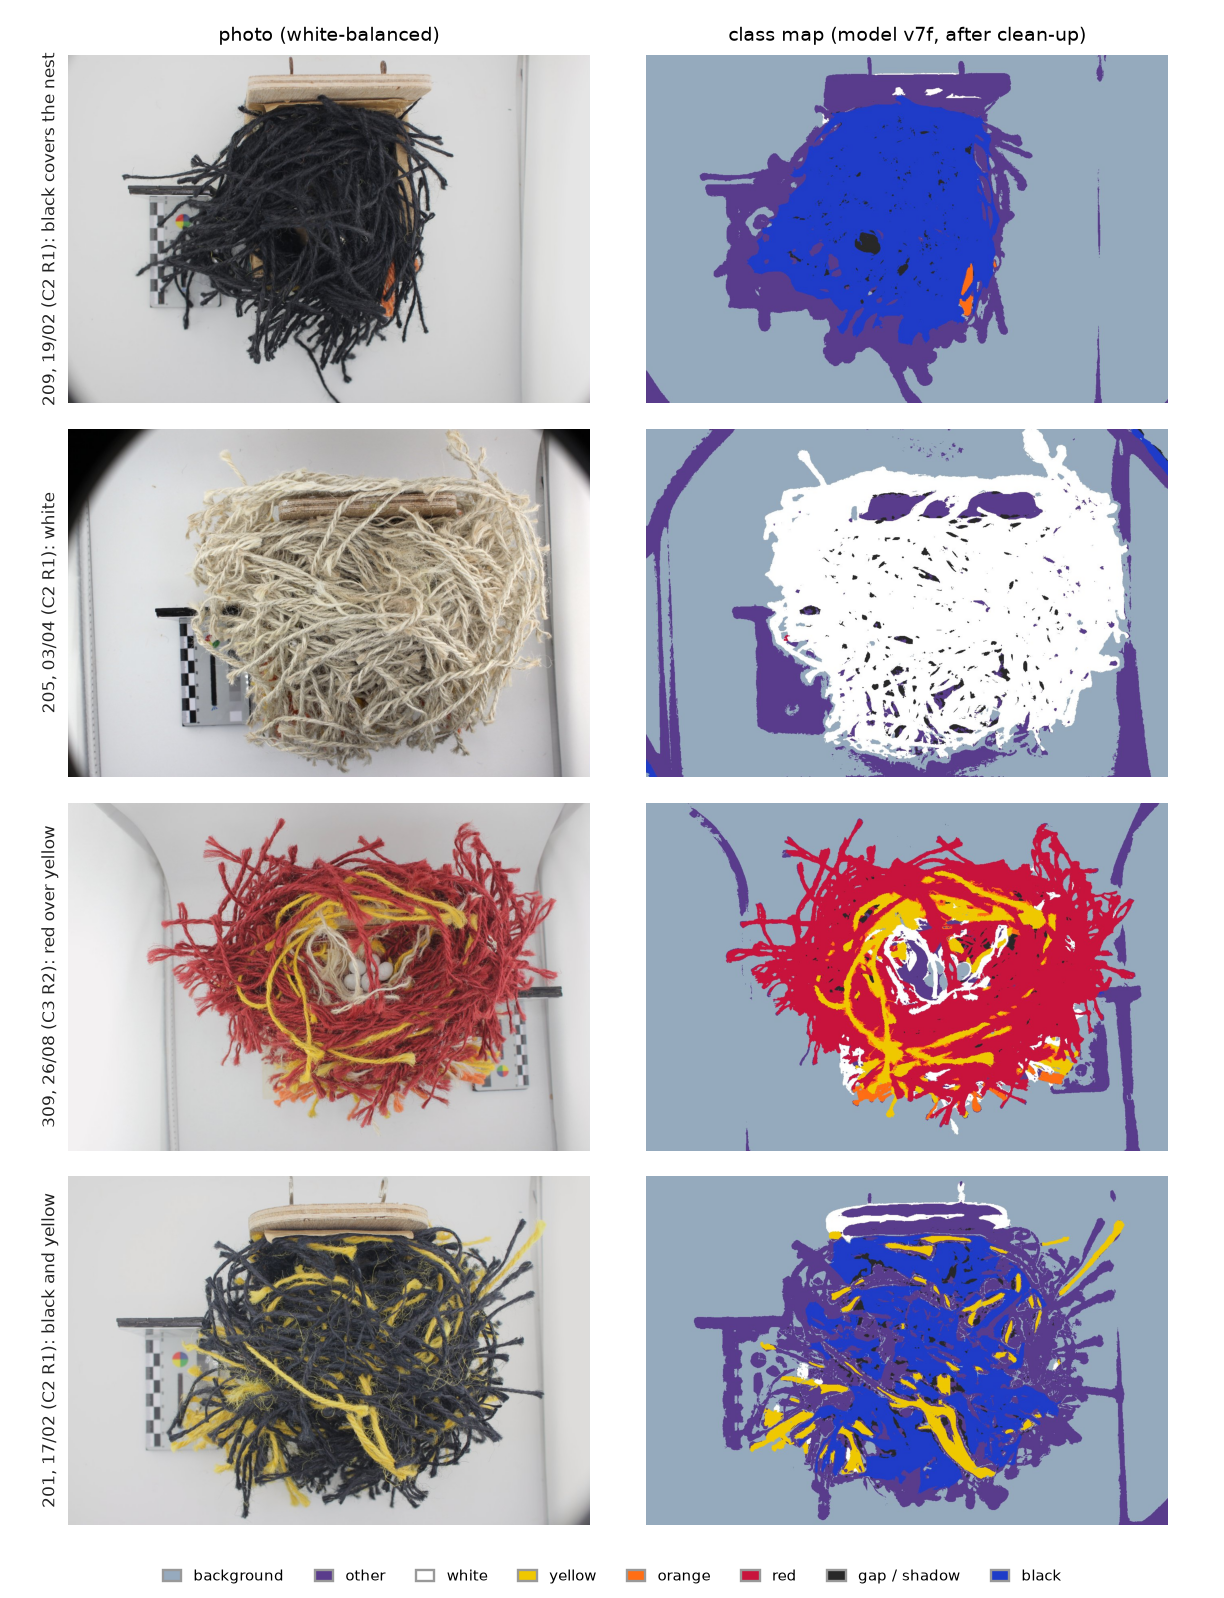
\includegraphics[width=0.92\textwidth]{figs/examples.png}
\caption{Segmentation of four top views of validation pairs (never used for training). Black string
is drawn in blue so that it differs from gap / shadow. Thin black strand tips at the edge of the nest
are sometimes labelled ``other'' (purple).}
\label{fig:examples}
\end{figure}

\section{Validation}

Points were drawn at random on the 105 top views of the 16 validation pairs, outside every training
rectangle, and shown one by one without the prediction (blind). Renaud labelled each point from a
context view and a zoom. 210 points were drawn uniformly over the nest (2 per photo), and 160 were
drawn among pixels of each predicted class (20 per class) so that rare classes such as black can also
be scored. \valnunsure{} answers (\valpunsure\,\%) were ``unsure'' (strand edges, blur) and are left out.

\begin{itemize}\setlength\itemsep{1pt}
\item Overall accuracy, uniform points: \textbf{\valacc} [95\,\% CI \valacclo--\valacchi], $n=\valnuniform$.
If every unsure uniform point were an error, it would be \valworst.
\item When both the annotator and the model see a coloured string, the colour is right in
\textbf{\valcolourok} of cases ($n=\valncolour$).
\item True string labelled gap / shadow (lost string): \vallost\,\%.
\end{itemize}

\begin{table}[H]
\centering\small
\begin{tabular}{lcccccc}
\toprule
& \multicolumn{3}{c}{precision: when the model says X, is it X?} & \multicolumn{3}{c}{recall: is a true X seen as X?} \\
\cmidrule(lr){2-4}\cmidrule(lr){5-7}
class & $n$ & rate & 95\,\% CI & $n$ & rate & 95\,\% CI \\
\midrule
\csname @@input\endcsname tables/validation_classes.tex 
\bottomrule
\end{tabular}
\caption{Scores per class. Precision uses all points; recall uses the uniform points only. ``Not string''
merges background and other material. Most white errors are light wood or background labelled white,
so the white area is slightly overestimated. Gap / shadow is weak, but it enters no colour metric.}
\label{tab:validation}
\end{table}

The pre-set criteria (colour correct $\geq 0.9$, lost string $\leq 10\,\%$, black $\geq 0.8$) are met.
There is one annotator only, so inter-observer agreement remains to be measured.

\section{Metrics}
\label{sec:metrics}

All metrics are computed per photo, on the string pixels of the class map.

\paragraph{Composition and area.} Share of each colour in the visible string, number of colours present
($\geq 2\,\%$), Shannon diversity, and areas in cm$^2$ through the scale. The median visible string area is
\areamed\,cm$^2$ (range \areamin--\areamax).

\paragraph{Mixing index (spatial autocorrelation, approach~3 of the project document).} Take every pair of
string pixels exactly $d$ millimetres apart, horizontally, vertically or diagonally, and record
whether the two have different colours. Then
\begin{equation*}
M(d) = \frac{\text{share of pairs of different colours at distance } d}{1-\sum_i p_i^2},
\end{equation*}
where $p_i$ is the share of colour $i$. The denominator is the share of different-colour pairs expected
if the colours were placed at random (Simpson heterogeneity). This makes nests with different
compositions comparable, and accounts for the number of colours used. $M=0$: colours sit in patches
larger than $d$. $M=1$: at that distance the colours are as mixed as if placed at random. $M$ is
computed at 3, 6, 12, 24 and 48\,mm; a strand is about 3.2\,mm wide. It is not computed when the second
colour makes up less than 10\,\% of the string, because the denominator is then too small.

\paragraph{Cell entropy (approach~1).} The photo is cut into square cells of 6 to 102\,mm. In each cell
that is at least half string, we compute the Shannon entropy of the colours, then average over
cells and divide by the entropy of the whole nest. 0 means each cell holds one colour; 1 means each
cell is as mixed as the whole nest. Across photos, cell entropy at 26\,mm and $M(12\,\text{mm})$ rank the
photos almost identically (Spearman \spearmixcell), so the two approaches agree.

\begin{figure}[H]
\centering
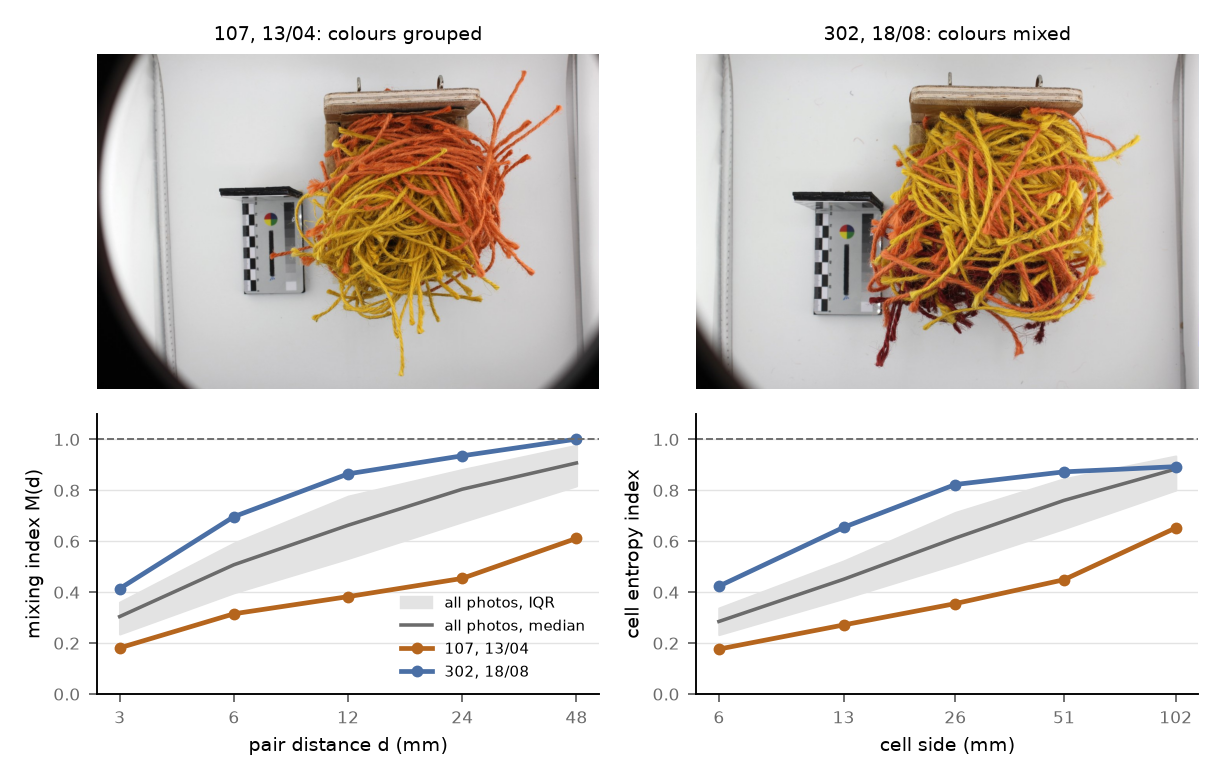
\includegraphics[width=\textwidth]{figs/mixing_example.png}
\caption{Two nests with nearly the same composition (yellow and orange; Simpson heterogeneity
\exAhet{} and \exBhet). Top: photos. Bottom: mixing index and cell entropy at increasing distances,
with the median and interquartile range of all photos. In 107 the colours form large patches
($M(12\,\text{mm}) = \exAmix$); in 302 the orange strands are scattered through the yellow
($M(12\,\text{mm}) = \exBmix$).}
\label{fig:mixing}
\end{figure}

\paragraph{Centre versus edge (stratification, top view).} For each string pixel, its position from the
edge of the nest (0) to the centre (1). Centrality is the mean position of each colour. $\rho$ is the
Spearman correlation, over the pixels of a photo, between provisioning rank (orange 1, yellow 2,
white 3, red or black 4) and position. $\rho>0$ means later colours lie closer to the centre.

\section{Results}

All results below use model v7f, whose segmentation was validated in the previous section. Statistics
use linear mixed models with a random intercept for the pair and a variance component for the nest
within the pair, since there are several photos per nest and two nests per pair. Fixed effects are
cohort, round, and days since the nest's first top photo (REML, \texttt{statsmodels}). The $p$-values are
not corrected for multiple tests.

\subsection{What the top view shows}

The top is dominated by the latest colour (Figure~\ref{fig:composition}). Nest 203 goes from all orange
to all black in five days, and in cohort~3 round~1 red covers 80--95\,\% of the top within one session.
A nest that looks yellow or white at its first top photo has covered its orange, not skipped it. The top
view therefore measures how the last layers are arranged, not the whole nest.

\begin{figure}[p]
\centering
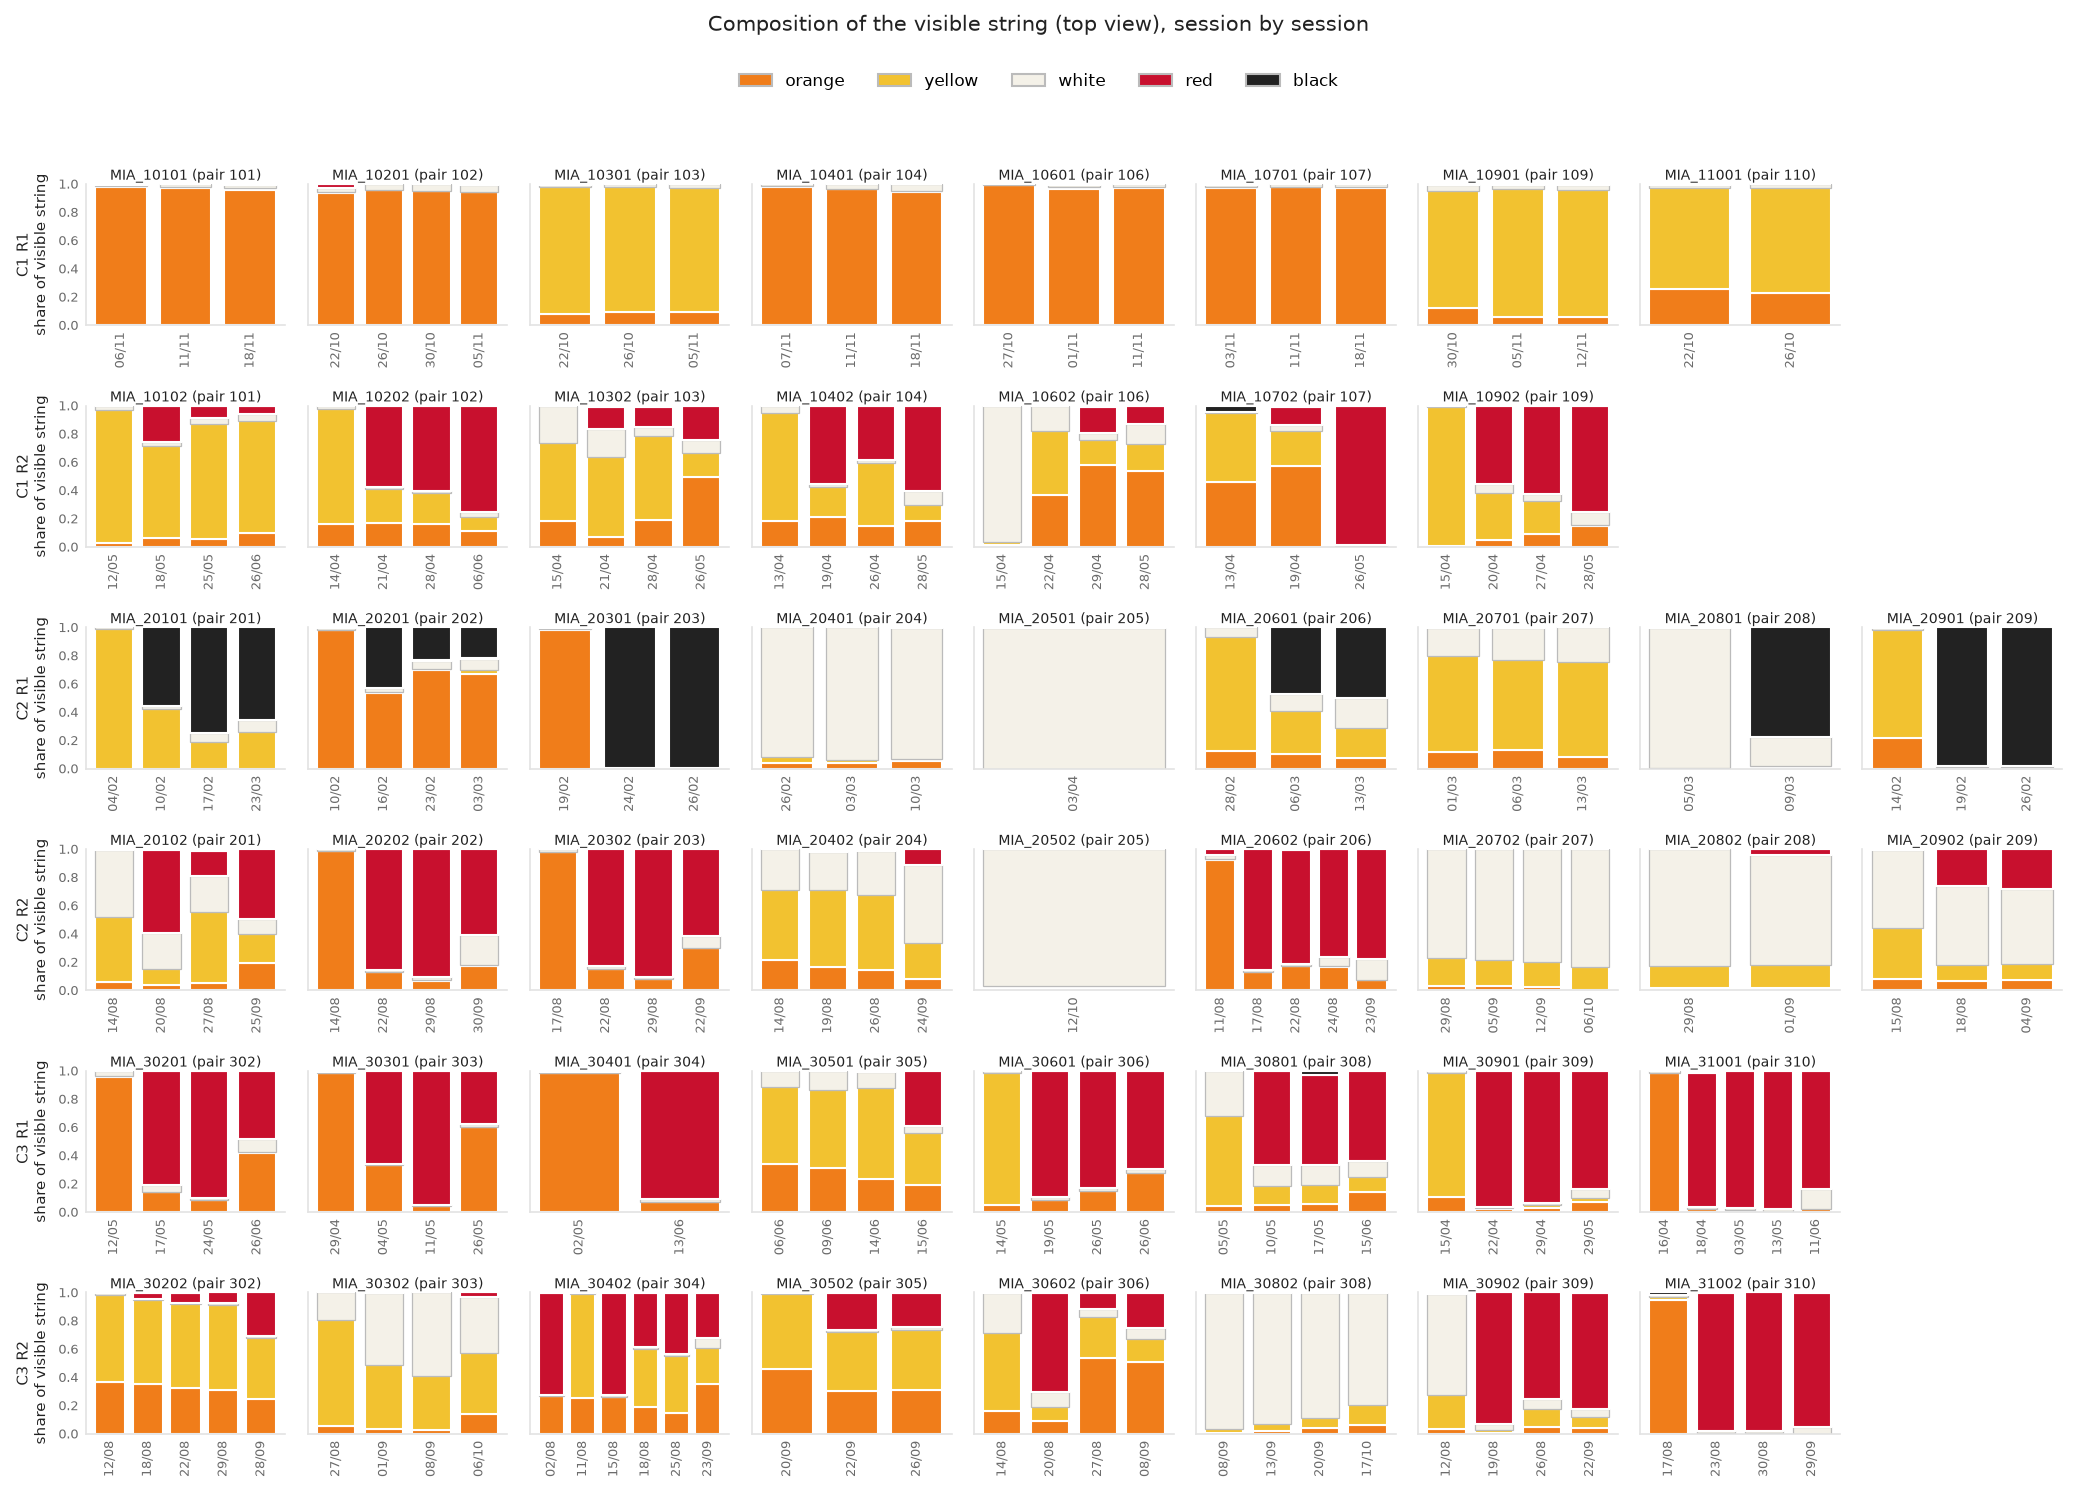
\includegraphics[width=\textwidth]{figs/composition.png}
\caption{Composition of the visible string for every nest (one panel per nest, one bar per session; rows:
cohort $\times$ round). Black appears only in cohort~2 round~1 and red never in cohort~1 round~1, as the
protocol expects. The only exceptions are below 5\,\% of the string, on three photos (two of them with dark vignetted corners).}
\label{fig:composition}
\end{figure}

\subsection{Mixing}

Colours form patches of a few centimetres. The median $M$ rises from \medmixthree{} at 3\,mm to
\medmixtwelve{} at 12\,mm and \medmixfortyeight{} at 48\,mm (Figure~\ref{fig:mixing}). Part of the low value
at short distances is mechanical: two points 3\,mm apart are often on the same strand, and pieces
are several centimetres long (see limitations). Nests differ widely: the median $M(12\,\text{mm})$ per nest
ranges from \nestmixmin{} to \nestmixmax{} over \nestmixn{} nests.

\begin{table}[H]
\centering\footnotesize
\resizebox{\textwidth}{!}{%
\begin{tabular}{lcccccc}
\toprule
& \multicolumn{2}{c}{mixing index, 12 mm} & \multicolumn{2}{c}{cell entropy, 26 mm} & \multicolumn{2}{c}{order--centre $\rho$} \\
\cmidrule(lr){2-3}\cmidrule(lr){4-5}\cmidrule(lr){6-7}
term & estimate [95\,\% CI] & $p$ & estimate [95\,\% CI] & $p$ & estimate [95\,\% CI] & $p$ \\
\midrule
\csname @@input\endcsname tables/models.tex
\bottomrule
\end{tabular}}
\caption{Linear mixed models (one row per photo). Variance shares are those of the random effects and the
residual.}
\label{tab:models}
\end{table}

Table~\ref{tab:models} uses one scale per index (12\,mm pairs, 26\,mm cells). Table~\ref{tab:scales}
repeats the model at every scale.

\begin{itemize}\setlength\itemsep{1pt}
\item \textbf{Second nests tend to be more mixed} than first nests. The effect is positive at all ten
scales (+0.02 to +0.08, largest around 12--26\,mm), but it reaches $p<0.05$ at one scale only (26\,mm cells,
$p=0.035$). With ten scales tested, this is a trend, not a result. Round is also confounded with the colours
available: every round-2 nest received red, while cohort~1 round~1 received nothing after the first egg.
\item No difference between cohorts, and no trend with time within a nest (Figure~\ref{fig:trends}).
\item \textbf{Where the variation lies.} The model splits the variation of the index into three levels:
  \begin{itemize}\setlength\itemsep{0pt}
  \item \emph{pair}: how much pairs differ on average. If it were large, the two nests of a pair would be alike;
  \item \emph{nest}: how much the two nests of the same pair differ;
  \item \emph{photo}: how much sessions of the same nest differ, including measurement error.
  \end{itemize}
  At 12\,mm, nests account for 44\,\% (about $\pm0.10$ on the index) and photos for 56\,\% (about $\pm0.11$). New
  string keeps covering the top between sessions, so photos of one nest vary a lot. Pairs account for 0\,\% at
  every scale: knowing the pair does not predict how mixed its nest is. A variance cannot be negative, so the
  estimate stops at 0. With few pairs this means ``not detectable'', not ``proven to be zero''
  (see Section~\ref{sec:signature}). The photo share grows with scale, because at large distances all nests
  approach random mixing and mostly session-to-session noise remains.
\end{itemize}

\begin{table}[H]
\centering\footnotesize
\begin{tabular}{llccc}
\toprule
index & scale & round 2 vs 1 [95\,\% CI] & $p$ & variance pair / nest / photo (\%) \\
\midrule
\csname @@input\endcsname tables/round_scales.tex
\bottomrule
\end{tabular}
\caption{Effect of round (2nd nest of the pair) at every scale of both mixing indices, from the same mixed model
as Table~\ref{tab:models} (cohort and days also included). The effect has the same sign everywhere, but is
weak and rarely significant.}
\label{tab:scales}
\end{table}

\begin{figure}[H]
\centering
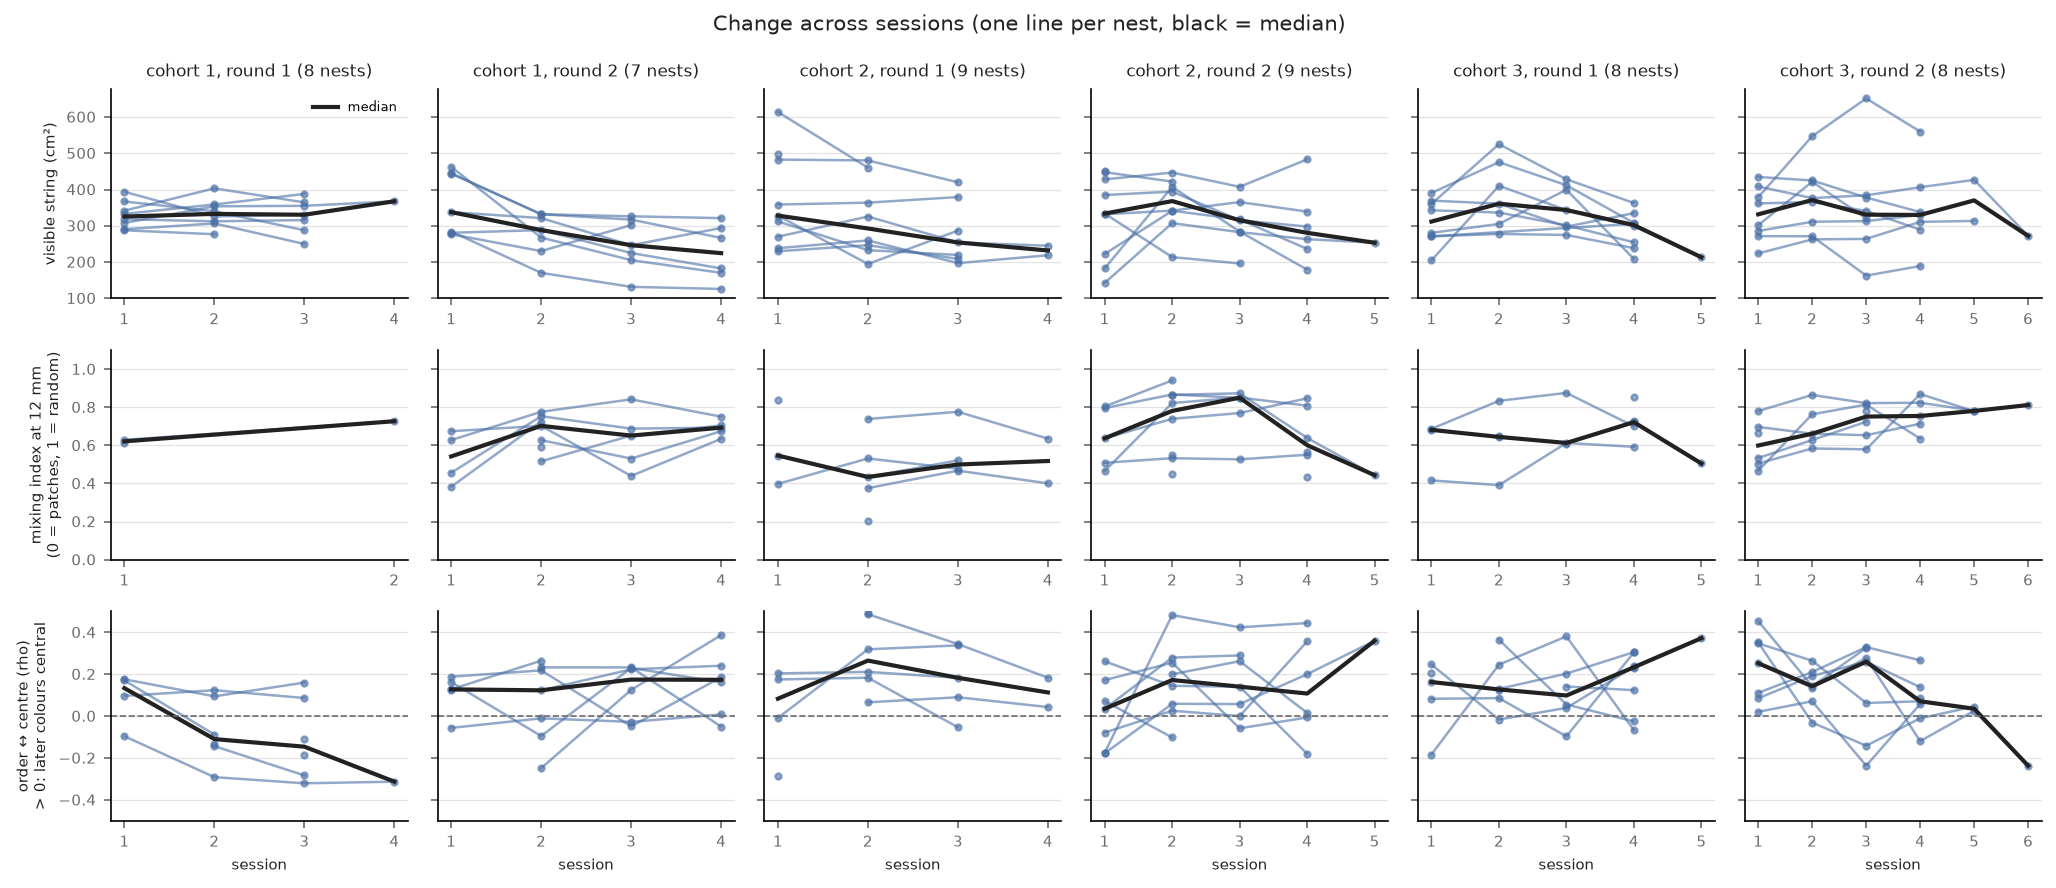
\includegraphics[width=\textwidth]{figs/trends.png}
\caption{Visible string area, mixing index at 12\,mm and order--centre $\rho$ across sessions (one line per
nest, black: median). Missing points: mixing not defined because one colour covers the top.}
\label{fig:trends}
\end{figure}

\subsection{Pair signature}
\label{sec:signature}

Do pairs have their own way of mixing, kept from one nest to the next? Repeatability was measured on the
mean per nest, for pairs where the metric is defined on both nests (Table~\ref{tab:rep},
Figure~\ref{fig:pairs}). There is no sign of it: repeatability is around zero, and so is the
correlation between first and second nests. With 13 pairs the confidence intervals are wide, so a
moderate repeatability (up to about 0.4) cannot be excluded. Pair 208 stands out: its first nest was
grouped (black over white), its second very mixed.

\begin{table}[H]
\centering\small
\begin{tabular}{lcccc}
\toprule
metric (mean per nest) & pairs & repeatability $R$ [95\,\% CI, bootstrap] & Spearman, nest 1 vs 2 & $p$ \\
\midrule
\csname @@input\endcsname tables/repeatability.tex 
\bottomrule
\end{tabular}
\caption{Repeatability of the pair (one-way intraclass correlation on nest means).}
\label{tab:rep}
\end{table}

\begin{figure}[H]
\centering
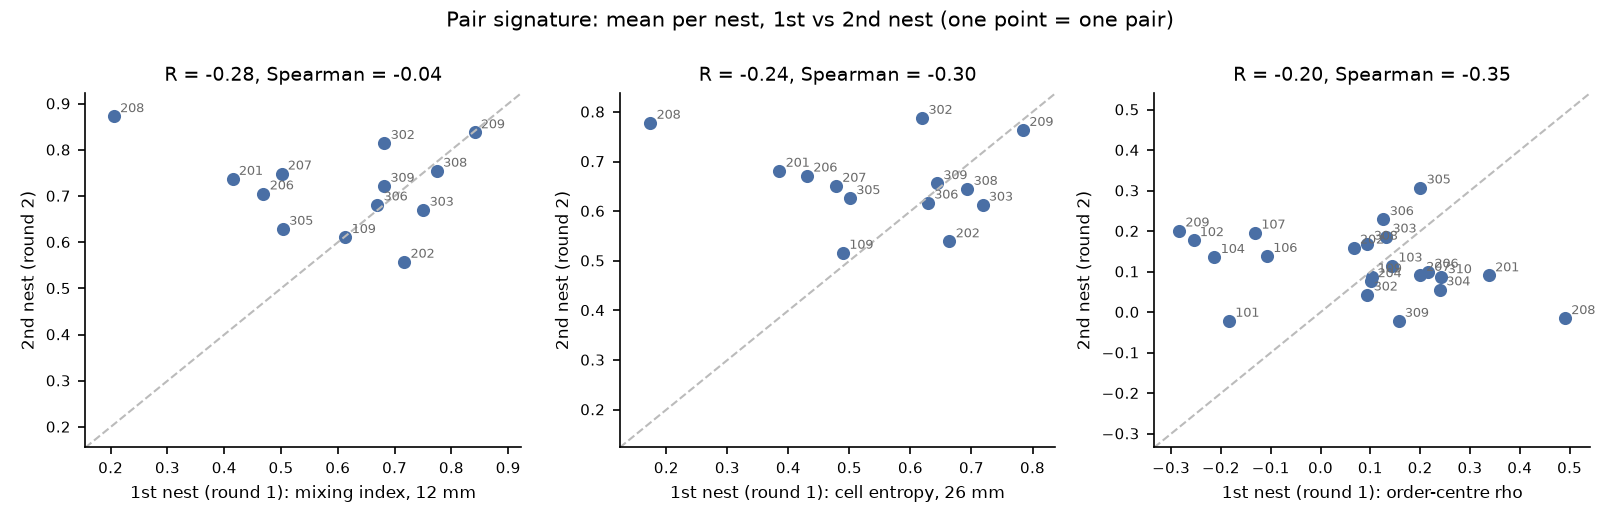
\includegraphics[width=\textwidth]{figs/pair_signature.png}
\caption{First versus second nest of each pair. Points on the diagonal would mean that a pair builds both
nests alike.}
\label{fig:pairs}
\end{figure}

\subsection{Later colours towards the centre}

Later colours are slightly closer to the centre of the cup. The mean $\rho$ is \rhomean{}
[95\,\% CI \rholo--\rhohi], and $\rho>0$ on \rhopos\,\% of \rhon{} photos. The effect is clearer in
cohorts~2 and~3 than in cohort~1 ($+0.10$ to $+0.11$, $p\approx0.02$; Table~\ref{tab:models}).
Per colour (Figure~\ref{fig:centrality}), orange is the most peripheral (median \centorange), and yellow
(\centyellow), red (\centred) and black (\centblack) are more central. White does not follow the order:
it is as peripheral as orange (\centwhite). Possible reasons are that white is often skipped, or
appears only as a thin rim around a red top; this is worth discussing.

\begin{figure}[H]
\centering
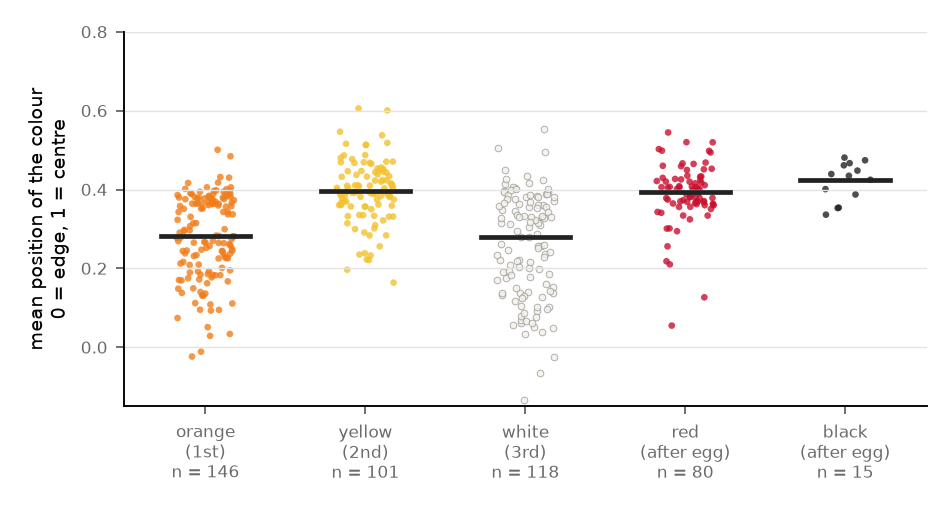
\includegraphics[width=0.75\textwidth]{figs/centrality.png}
\caption{Mean position of each colour per photo (where the colour makes up at least 2\,\% of the string);
bar: median.}
\label{fig:centrality}
\end{figure}

\section{Limitations}

\begin{itemize}\setlength\itemsep{1pt}
\item \textbf{The top view shows only the last layer.} Hidden colours, and stratification in height,
need the side views.
\item \textbf{Pixels, not strands.} A long strand weighs more than a short one. The mixing index is low at
short distances partly because neighbouring points lie on the same strand. Comparisons between nests
are valid, since all nests use the same string, but the absolute value of $M$ cannot be read as
``behaviour'' without a null model of randomly laid strands.
\item \textbf{Mixing is undefined when one colour covers the top}, which removes most of cohort~1 round~1.
\item \textbf{Round is confounded with the colours available} (red in every round-2 nest).
\item One annotator for the validation; $p$-values not corrected for multiple testing.
\end{itemize}

\section{Next steps}

\begin{enumerate}\setlength\itemsep{1pt}
\item \textbf{A null model by simulation}: lay strands of the real length and width at random, with each nest's
composition and footprint, and compare its mixing curve with the real one. This separates behaviour from
strand geometry. It needs the length of the string pieces.
\item \textbf{Side views} (345 photos, same nests and sessions): stratification in height, measured in mm above
the cage grid (a fixed reference), and the colours hidden under the top layer. The colour stage already
works on side views; the string-detection stage needs about 10--15 annotated side views and retraining.
\item A second annotator on part of the validation points, for inter-observer agreement.
\end{enumerate}

\paragraph{Reproducibility.} Scripts are in \texttt{scripts/}:
\begin{itemize}\setlength\itemsep{0pt}
\item \texttt{top\_metrics.py}: segmentation and metrics;
\item \texttt{stats\_top.py}: models;
\item \texttt{make\_top\_report.py}: all figures and numbers of this report.
\end{itemize}
Per-photo metrics: \texttt{outputs/top/metrics\_v7f.csv}.

\end{document}
